\documentclass[problem]{mcs}

\begin{pcomments}
  \pcomment{PS_koch_snowflake}
  \pcomment{from: S06.ps3}
\end{pcomments}

\pkeywords{
  recursion
  structural_induction
  fractal     
}

%%%%%%%%%%%%%%%%%%%%%%%%%%%%%%%%%%%%%%%%%%%%%%%%%%%%%%%%%%%%%%%%%%%%%
% Problem starts here
%%%%%%%%%%%%%%%%%%%%%%%%%%%%%%%%%%%%%%%%%%%%%%%%%%%%%%%%%%%%%%%%%%%%%

\begin{problem}
  Fractals are example of a mathematical object that can
  be defined recursively.  In this problem, we consider the Koch
  snowflake.  Any Koch snowflake can be constructed by the following
  recursive definition.
  \begin{itemize}

  \item \textbf{base case}: An equilateral triangle with a positive
    integer side length is a Koch snowflake.

  \item \textbf{constructor case}: Let $K$ be a Koch snowflake, and
    let $l$ be a line segment on the snowflake.  Remove the middle
    third of $l$, and replace it with two line segments of the same
    length as is done in Figure~\ref{kochline}

    The resulting figure is also a Koch snowflake.
  \end{itemize}

  Prove by structural induction that the area inside any Koch
  snowflake is of the form $q\sqrt{3}$, where $q$ is a rational
  number.

\begin{solution}
    We first show that the side length of any Koch snowflake
    is rational, and prove it in the lemma below.

    \begin{lemma*}
      Every side length of a Koch snowflake is rational.
    \end{lemma*}

    \begin{proof}
      For the base case, every side length is the same positive
      integer.  For the inductive case, let $K$ be a Koch snowflake.
      Then $K$ was constructed by modifying a Koch snowflake $K'$ as
      in the recursive case.  By the induction hypothesis, each side
      length of $K'$ is rational.  Let $l$ be the line segment of $K'$
      modified via the recursive case.  The two new line segments are
      of length $\frac{l}{3}$, which is rational since $l$ is
      rational.
    \end{proof}

    Now, we prove the main theorem.
    \begin{proof}
      We prove the claim by structural induction.

      For the base case, the area of an equilateral triangle with side
      length $l$ is $q\sqrt{3}$, where $q = \frac{l}{2}$.

      For the inductive case, let $K$ be a Koch snowflake.  $K$ was
      constructed by modifying a Koch snowflake $K'$ as in the recursive
      case above.  By the induction hypothesis, the area of $K'$ is
      $q\sqrt{3}$ for some rational $q$.  Let $l'$ be the length of the
      line segment of $K'$ that was modified according to the recursive
      case.  The area added by the modification is $q' \sqrt{3}$, where
      $q' = \frac{l'}{6}$.  By the above lemma, $l'$ is rational, so
      $q'$ is rational.  Thus, the area of $K$ is $(q' + q) \cdot
      \sqrt{3}$, and $q' + q$ is rational, so we have proved our claim.
    \end{proof}
\end{solution}

    \begin{figure}
      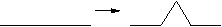
\includegraphics[width=2.5in]{koch}
     \caption{Constructing the Koch Snowflake.}
     \label{kochline}
    \end{figure}

\end{problem}

%%%%%%%%%%%%%%%%%%%%%%%%%%%%%%%%%%%%%%%%%%%%%%%%%%%%%%%%%%%%%%%%%%%%%
% Problem ends here
%%%%%%%%%%%%%%%%%%%%%%%%%%%%%%%%%%%%%%%%%%%%%%%%%%%%%%%%%%%%%%%%%%%%%

\endinput

